\chapter{Проектирование базового RAG-ассистента RobyMAX}
\label{chapter:architecture}

\section{Требования к прототипу}

Первая MVP-версия должна реализовывать полный минимальный путь от исходных документов до ответа на пользовательский вопрос. К функциональным требованиям относятся:
\begin{compactenum}
  \item загрузка и учет исходных документов;
  \item парсинг документов разных форматов и приведение текста к единому виду;
  \item разбиение документов на чанки;
  \item построение embeddings для чанков;
  \item индексация чанков в Qdrant;
  \item прием пользовательского вопроса;
  \item поиск top-k релевантных чанков;
  \item генерация ответа на основе найденного контекста;
  \item возврат списка источников и \texttt{chunk\_id}.
\end{compactenum}

К нефункциональным требованиям относятся локальная воспроизводимость, модульность, работа с русскоязычными документами, возможность дальнейшего расширения и минимальная зависимость от внешних API. Для учебно-исследовательской работы также важно, чтобы каждый этап оставлял проверяемые артефакты: реестр, parsed-корпус, чанки, embeddings, manifest-файлы и отчеты.

\section{Архитектура обработки документов}

Архитектура обработки документов строится как offline-конвейер. Его задача — подготовить данные до момента пользовательского запроса. Исходные файлы располагаются в \path{data/raw}. Для них формируется реестр \path{data/registry/documents_registry.csv}, где фиксируются устойчивые идентификаторы, категория, формат файла и путь к источнику. Реестр нужен для воспроизводимости: при повторной обработке документы сохраняют стабильные \texttt{doc\_id}.

После регистрации документы парсятся в структурированный JSONL-корпус \path{data/parsed/documents.jsonl}. Парсинг отделяет извлечение текста от последующих этапов. Это позволяет одинаково работать с DOCX, PDF и XLSX после приведения их к общему представлению блоков. Валидация parsed-корпуса проверяет отсутствие пустых и некорректных записей. По отчету \path{data/reports/parsing/parsed_corpus_validation.json} для текущего корпуса зафиксировано 0 ошибок и 0 предупреждений.

Затем parsed-блоки преобразуются в чанки. В проекте используется целевой размер чанка 1500 символов и максимальный размер 2500 символов. Такой выбор является компромиссом: слишком короткие фрагменты могут потерять контекст, а слишком длинные ухудшают точность поиска и увеличивают вход LLM. Перекрытие в один блок используется для сохранения связи между соседними фрагментами. По отчету \path{data/reports/chunking/chunking_report.json} сформирован 481 чанк, средний размер составил 1245.99 символа, а чанков сверх максимального ограничения не обнаружено.

Для каждого чанка строится embedding. Матрица embeddings сохраняется в \path{data/processed/chunk_embeddings.npy}, а связь между строкой матрицы и \texttt{chunk\_id} хранится в \path{data/processed/chunk_embeddings_manifest.jsonl}. Такое разделение числовых данных и metadata упрощает проверку, повторную индексацию и диагностику ошибок.

\begin{figure}[h]
\centering
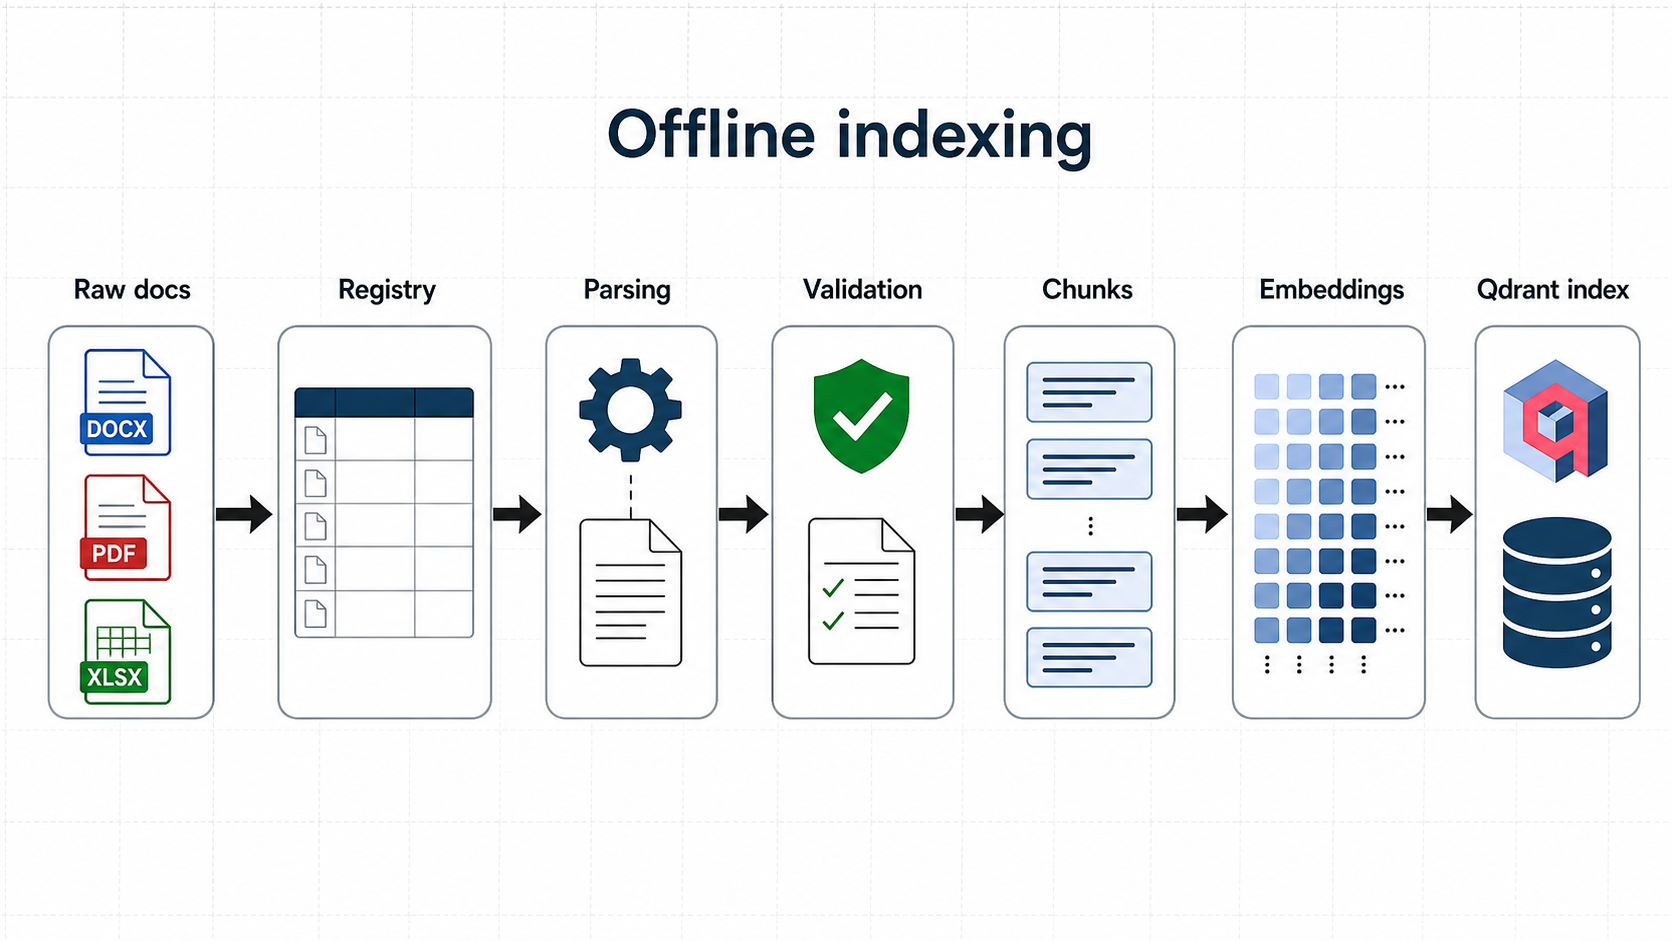
\includegraphics[width=\textwidth]{img/generated/rag_offline_indexing.png}
\caption{Алгоритм подготовки и индексации документов в MVP}
\label{fig:mvp-offline-indexing}
\end{figure}

Схема на рисунке~\ref{fig:mvp-offline-indexing} отражает offline-этап: от исходных документов до Qdrant-индекса. После его выполнения система готова отвечать на вопросы без повторного парсинга и векторизации корпуса.

\section{Архитектура поиска}

В первой MVP-версии используется только dense retrieval. Пользовательский вопрос кодируется той же embedding-моделью, что и чанки корпуса. Полученный вектор передается в Qdrant, после чего система получает top-k ближайших чанков. Каждый найденный чанк содержит текст и payload, включающий \texttt{chunk\_id}, \texttt{doc\_id}, путь к исходному файлу, категорию, заголовки и другие сведения, необходимые для формирования контекста и вывода источников.

В репозитории уже присутствуют более развитые механизмы поиска, однако в рамках первой пояснительной записки они не рассматриваются как основной результат. Граница MVP проводится по базовой схеме dense retrieval: один embedding вопроса, поиск ближайших векторов в Qdrant и передача найденных фрагментов в генерацию.

\section{Архитектура генерации ответа}

После retrieval найденные чанки упаковываются в контекст. Контекст должен быть достаточно полным, чтобы LLM могла сформировать ответ, но не должен превышать допустимый размер входа модели. Поэтому при упаковке ограничивается общий объем контекста и максимальная длина одного чанка. Это снижает риск передачи лишнего шума и делает генерацию более предсказуемой.

Prompt задает модель поведения: отвечать на русском языке, использовать только предоставленный контекст, не придумывать отсутствующие сведения, при недостатке информации явно сообщать об этом и возвращать источники. Генерация выполняется локальной моделью через OpenAI-compatible API, что отделяет код RAG-пайплайна от конкретного backend LLM.

\begin{figure}[h]
\centering
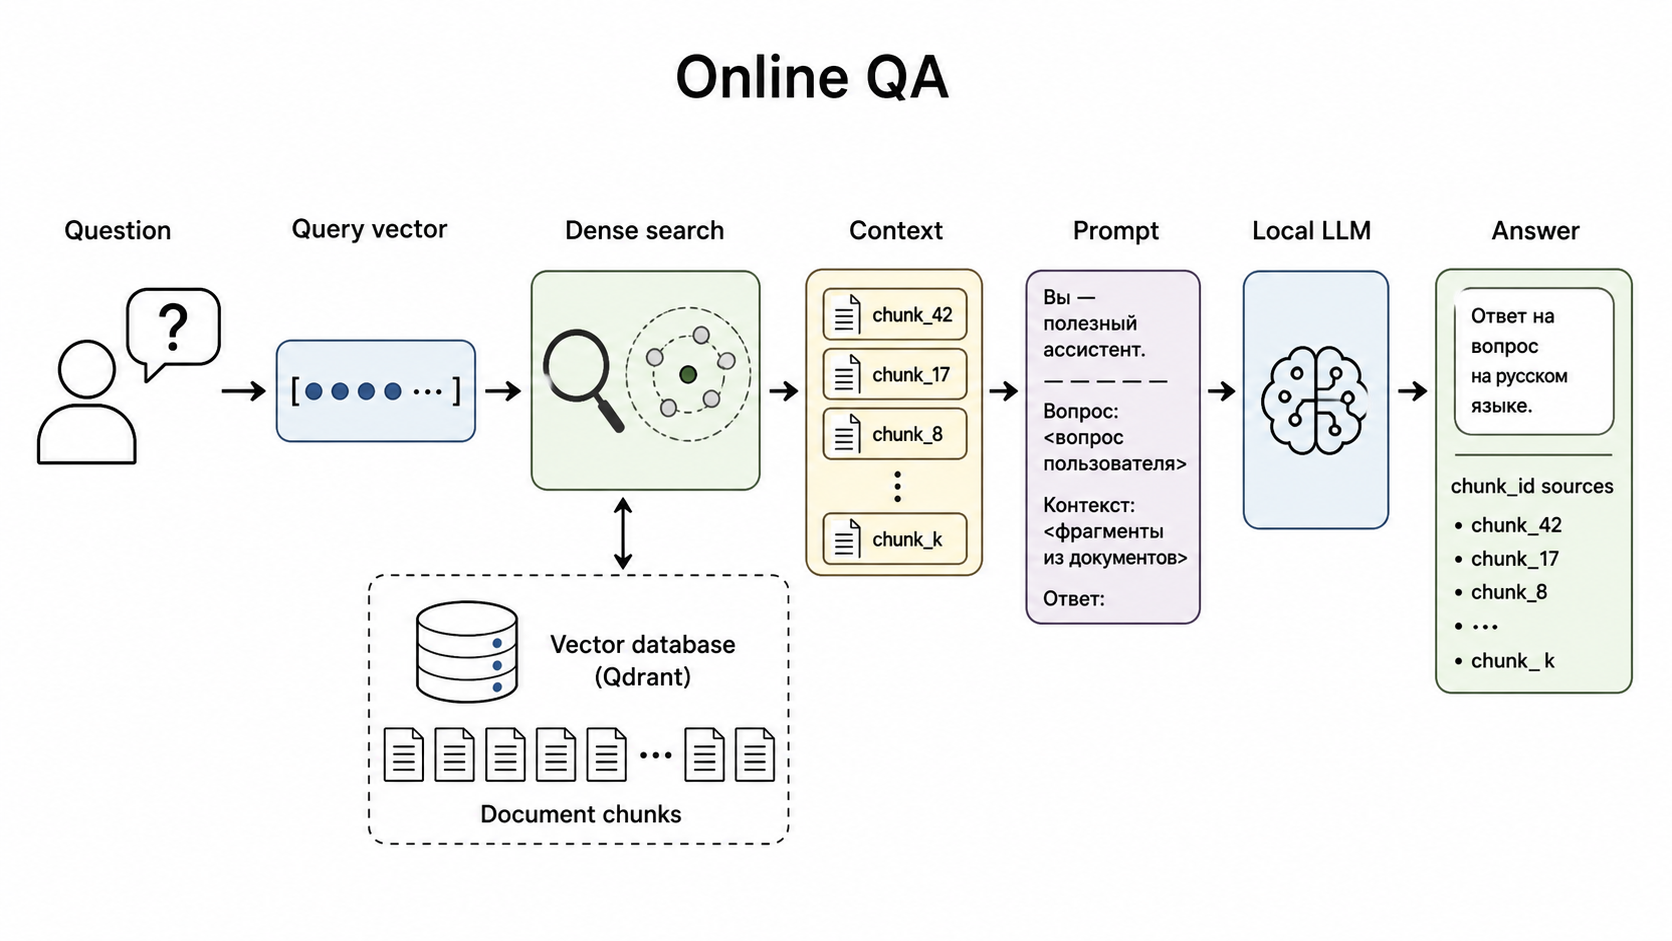
\includegraphics[width=\textwidth]{img/generated/rag_online_answer.png}
\caption{Алгоритм обработки пользовательского запроса в MVP}
\label{fig:mvp-online-answer}
\end{figure}

На рисунке~\ref{fig:mvp-online-answer} показан online-этап. Вопрос пользователя преобразуется в вектор, затем выполняется dense search по Qdrant, найденные чанки образуют контекст, после чего LLM формирует ответ и список источников.

\section{Выводы по главе}

Спроектирован базовый RAG-ассистент, состоящий из двух частей: offline-конвейера подготовки документов и online-конвейера ответа на вопрос. В первой MVP-версии центральными компонентами являются embeddings, Qdrant, dense retrieval, context packing и LLM. Архитектура оставляет возможность дальнейшего расширения, но основной результат первой версии ограничен проверяемым dense RAG-сценарием.

%%% Local Variables:
%%% TeX-engine: xetex
%%% End:
